\chapter{General framework of \smtrat}
\label{chapter:generalframework}


Our toolbox has a modular \Cpp class design which can be used to
compose NRA theory solvers for an SMT embedding in a \emph{dynamic} and \emph{hierarchic} fashion.
Our NRA theory solvers are instances of \managerClass,
which offers an interface to communicate with the environment and
which coordinates the satisfiability check according to a user-defined
\strategyClass. Such a strategy combines basic NRA theory solver modules, derived from \moduleClass.
% NRA theory problems are specified using the \formulaClass
% class. Basic NRA theory solver modules are derived from the
% \moduleClass class. Such modules can be embedded into a \managerClass,
% which offers an interface to communicate with the environment and
% which coordinates the satisfiability check according to a user-defined
% \strategyClass.
Figure~\ref{fig:framework} shows an example configuration.
Moreover, a \Java-based graphical user interface (GUI) can be
used for an intuitive and user-friendly specification of strategies
(and the automatic generation of a corresponding \strategyClass
class).
Next, we briefly describe these concepts. 

\section{The \formulaClass class}
\formulaClass instances contain, besides a sequence of NRA
constraints, a bitvector storing some information about the problem
and the history of its check.  E.g., there is a bit which is 
$1$ if some of the constraints are equations. Also for each module
there is a bit which is $1$ if the module was already invoked
on the given problem. Such information can be used
to specify conditions under which a procedure should be invoked for
a certain problem.\smallskip

\section{The \moduleClass class}
A \emph{module} is an SMT-compliant implementation of a procedure
(e.g., constraint simplifier, an incomplete procedure or a complete decision
procedure) which can be used for the satisfiability check of NRA formulas. 
A module's interface allows to add 
constraints, to push and pop backtrack points, to check the so far
added constraints for consistency and to obtain an infeasible subset
of these constraints if they are detected to be inconsistent.

Modules have the opportunity to call other modules (\emph{backends})
on sub-problems. A novel achievement of our toolbox is that this call
hierarchy is \emph{dynamic} and guided by a \emph{user-defined
  strategy}. Currently, we only support sequential execution, parallel
solving is planned for later releases.

Inheritance can be used to extend existing modules.
Besides the basic type \moduleClass, our toolbox offers
five sub-classes. \simplifierModuleClass
(\simplifierModule) implements smart simplifications, whereas
\groebnerModuleClass (\groebnerModule) simplifies equation systems 
using Gr\"obner bases and probably detects inconsistency. The 
cylindrical algebraic decomposition method is implemented in
\univariateCADModuleClass (\univariateCADModule) for the
univariate case and in \cadModuleClass (\CADModule) for the general
multivariate case. The last module class \vsModuleClass (\vsModule)
implements a version of the virtual substitution method.\smallskip

\begin{figure}[t]
\caption{A snapshot of an \smtrat composition embedded in an SMT solver.}
\begin{center}
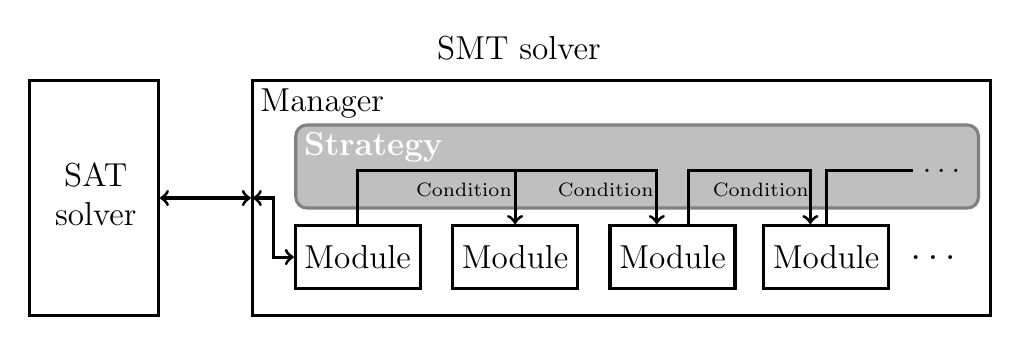
\begin{tikzpicture}[every node/.style={rectangle}, text centered, bend angle=15, scale=1, line width=.4mm]
	\node[] (smtsolver) at (-2.5, 2.2) {\large SMT solver};
	\node[draw, minimum height=85pt, text width=40pt] (satsolver) at (-7.9, 0.3) {\large\begin{tabular}{c}SAT \\ solver\end{tabular}};
	\node[draw, minimum height=85pt, text width=260pt] (manager) at (-1.2, 0.3) {};
	\node[] (managerText) at (-5, 1.5) {\large Manager};
	\node[fill=lightgray,draw=gray, rounded corners, minimum height=30pt, text width=240pt] (strategy) at (-1,.7) {};
	\node[] (strategyText) at (-4.35, .95) {\large\bf \color{white} Strategy};
	\draw[<->] (-5.36,-.45) -- (-5.62,-.45) -- (-5.62,.3) -- (-5.88,.3);
	\draw[->] (-4.55,-.03) -- (-4.55,.65) -- (-.75,.65) -- (-.75,-.03);
	\node[] (strategyText) at (-1.4, .4) {\scriptsize Condition};
	\draw[->] (-2.55,.65) -- (-2.55,-.03);
	\node[] (strategyText) at (-3.2, .4) {\scriptsize Condition};
	\draw[->] (-.35,-.03) -- (-0.35,.65) -- (1.2,.65) -- (1.2,-.03);
	\node[] (strategyText) at (.57, .4) {\scriptsize Condition};
	\draw (1.4,-.03) -- (1.4,.65) -- (2.5,.65);
	\node[] (dotsa) at (2.9,.65) {\large \ldots};
	\node[draw, minimum height=23pt] (moduleAText) at (-4.55, -.45) {\large Module};
	\node[draw, minimum height=23pt] (moduleBText) at (-2.55, -.45) {\large Module};
	\node[draw, minimum height=23pt] (moduleCText) at (-.55, -.45) {\large Module};
	\node[draw, minimum height=23pt] (moduleDText) at (1.4, -.45) {\large Module};
	\node[] (dotsc) at (2.8, -.45) {\Large \ldots};
	\path[<->] (satsolver.0) edge[] node[left] {} (manager.180);
\end{tikzpicture}

\end{center}
\label{fig:framework}
\end{figure}

\section{The \strategyClass class}
\smtrat offers a framework to integrate
single modules to powerful and efficient \emph{composed theory solvers}. 
%\emph{TODO: Results and reasons why the composition is faster.}
The composition relies on a user-defined 
\strategyClass that specifies for each
\formulaClass instance which module should be used for its check.  A strategy is basically a sequence
of condition-module pairs. For each \formulaClass instance, it determines the first
module whose condition evaluates to true on the bitvector of the formula.
E.g., the strategy
``$c_1\ ?\ (m_1)\ :\ (c_2\ ?\ (m_2)\ :\ (m_3))$''
determines $m_1$ as module type for $\varphi$
if the bitvector of $\varphi$ fulfills the condition $c_1$. If $\varphi$ does 
not fulfill $c_1$ but $c_2$, then an instance of $m_2$ is called,
otherwise of $m_3$.\smallskip

\section{The \managerClass class}
The \managerClass contains references to the available module
instances and to the user-defined strategy.  It manages, on the one
hand, the creation and linking of the modules, and, on the other hand,
the communication between them and the environment, e.g., the frontend of an
SMT solver. 

